\bigbreak

\lettrine{I}{n} the last chapter we have introduced the framework of network science used to study the brain networks. We showed that the modular organization of brain networks has been widely investigated using graph theoretical approaches and demonstrated that graph partitioning methods based on the maximization of global fitness functions, like Newman's Modularity, suffer from a fundamental resolution limit as they fail to detect modules that are smaller than a scale determined by the size of the entire graph.
We explored the effects of this limitation on the study of brain connectivity networks, demonstrating that the resolution limit prevents detection of important details of the brain modular structure, thus hampering the ability to appreciate differences between networks and to assess the topological roles of nodes.
Additionally, the question whether 

To this end, we will show that Surprise\index{Surprise}, a recently proposed fitness function based on probability theory, does not suffer from these limitations.
Surprise maximization in brain co-activation and functional connectivity resting state networks reveals the presence of a rich structure of heterogeneously distributed modules, and differences in networks' partitions that are undetectable by resolution-limited methods.
Moreover, Surprise leads to a more accurate identification of the network's connector hubs, the elements that integrate the brain modules into a cohesive structure. 
In this chapter we will introduce Surprise from its theoretical foundations and discuss its properties in details. Finally, an explicitly made algorithm for Surprise optimization in binary graphs is presented, with a comparison of its performance on benchmark networks.

\section{Binary networks}
\subsection{A probabilistic interpretation of community detection}\label{sec:probability_clustering}
As previously described, no spin-glass based additive quality function, including Newman's Modularity, is by any means measuring the statistical significance of the deviation between the fraction of edges falling within modules and the null model.
In other terms, no spin-glass based quality function is telling us the level of statistical confidence at which one should discard the null hypothesis that the observed fraction of edges inside a community is the same as the one expected from a given null model.

To address this question, one should instead compute probabilities, as they are the natural way to measure statistical significance.
Specifically, given a node induced subgraph (a community), one is interested in computing the probability to find another subgraph having more internal edges than the observed one: the lesser the value, the more significant is the community in exam. Surprise can be thought as a quality function that moves away from the framework of additive functions based on spin-glass models, as described in the previous chapter and tries to address these questions quantitatively.
Precisely, the problem is the following: given a subgraph, what is the probability of observing another subgraph with a larger number of internal edges drawn from a random graph with a given density?
This question is answered by the urn model in classical probability theory. The reason is clear if one imagines that each pair of nodes is a marble, which is one color if the nodes are connected by a link and the other color if they are not.
A number of marbles is drawn from an urn without replacement and the probability of observing a given number of marbles of one specific color is calculated by means of the hypergeometric law.
When applied to clustering, the problem corresponds to the calculation of the probability to observe a fixed number of internal edges in a randomly drawn set of nodes defining a community.
For example, suppose that one draws a subgraph with $n_c$ nodes, $p_c$ pairs of nodes and $m_c$ edges from a graph with $n$ nodes, $p$ pairs of nodes and $m$ edges (see Section for the notation~\ref{sec:clustering}).
As indicated by the urn model, the probability to observe exactly $m_c$ internal edges is given by:
\begin{equation}\label{eq:subgraph_probability}
\Pr[i=m_c] = \frac{\binom{m}{i}\binom{p-m}{p_c-i} }{\binom{p}{p_c}} = \frac{\binom{p_c}{i} \binom{p-p_c}{m-i}}{\binom{p}{m}}
\end{equation}
where the last equality is because of the Vandermonde identity~\cite{feller1968}.
The probability in Eq.~\ref{eq:subgraph_probability} is simply understood in terms of urn model as there are $\binom{p_c}{i}$ ways of choosing exactly $i$ black marbles from a population of $p_c$ black marbles, $\binom{p-p_c}{m-i}$ ways of choosing $(m-i)$ white marbles from a population of $(p-p_c)$ white marbles and a total possible number of combinations of $m$ marbles taken from a population of $p$ of them.
As the probability of observing $i$ or more internal edges, is given by the sum of the probabilities of observing exactly $i$,$i+1$,$i+2$ etc. internal edges, summing on $i$ yields the probability of getting \emph{at least} $m_c$ white marbles:
\begin{equation}\label{eq:subgraph_probability_marginalized}
\Pr[ m_c \geq i ] = \sum\limits_{i=m_c}^{m} \frac{\binom{p_c}{i} \binom{p-p_c}{m-i}}{\binom{p}{m}}
\end{equation}

In this last equation we are considering the probability of randomly drawing a subgraph with $m_c$ or more internal edges over the set of all random subgraphs with $n$ nodes and exactly $m$ edges as in the $G_{nm}$ model described in section~\ref{sec:models_random_graph}. Indeed, the denominator $\binom{p}{m}$ in Equation~\ref{eq:subgraph_probability_marginalized} represent the possible number of graphs with $p$ pairs of nodes and $m$ edges. 

\section{Surprise}
The intuition of Eq.~\ref{eq:subgraph_probability_marginalized} gets very close to the definition of Surprise given by Aldecoa and Marin~\cite{aldecoa2011}, giving to Surprise a clearer theoretical motivation that to the best of our knowledge, did not appear in any other work. Hence, if we consider as the random subgraph that is drawn from the $G_{n,m}$ set, one with at least $m_\zeta=\sum_c m_c$ internal edges and $p_\zeta=\sum_c p_c$ pairs of edges, then such subgraph represents a whole clustering. In this case, the definition given in Eq.~\ref{eq:subgraph_probability_marginalized} and the definition given in~\cite{aldecoa2011} are perfectly equivalent. Indeed, for a partition $\zeta$, the probability that a subgraph $\mathcal{G}$ randomly drawn from the set $G_{nm}$ has at least $m_\zeta$ intracluster edges and $p_\zeta$ intracluster pairs is modeled after the inverse cumulative hypergeometric distribution, exactly as in~\ref{eq:subgraph_probability_marginalized}.
Here and in the rest of the work, we dub \emph{Surprise} the following probability:
\begin{equation}\label{eq:surprise}
S(\zeta) := \sum_{i = m_\zeta}^m \dfrac{\binom{p_\zeta}{i} \binom{p-p_\zeta}{m-i} }{\binom{p}{m}}
\end{equation}

Surprise computes the probability to (surprisingly) observe at least as many internal edges as within the proposed partition in a uniform random graph.
As mentioned, model in Eq.~\ref{eq:surprise}  corresponds to an urn model without reinsertion, where $S$ is the probability of extracting at least $m_\zeta$ white balls out of $m$ trials from an urn containing $p_\zeta$ white balls and $p-p_\zeta$ black balls.
Intuitively, the lower $S(\zeta)$, the better the clustering. Optimal partitions with respect to $S$ are those with the highest number of intracluster edges and the smallest number of intracluster pairs. 

Differently from Modularity, $S(\zeta)=1$ both for the partition where every node is in a separated community ($|C|=n$,$p_\zeta=0$,$m_\zeta=0$) and for the partition that entails all nodes into a single group ($|C|=1$,$p_\zeta=p$,$m_\zeta=m$) as is evident from its formulation in terms of urn model. Indeed, as Newman's Modularity is zero when $C=1$, it is different than zero in the case $C=n$. In this sense Surprise is a more meaningful quality function as both the extremal partitions are uninteresting, yielding zero Surprise.

It should be noted that due to numerical precision problems in the evaluation of large binomial coefficients, $\hat{S}(\zeta) := -\log_{10}S(\zeta)$ is often taken as measure of quality of the partition, which is totally equivalent with respect to optimum solutions, where higher values correspond to better clustering.
Different authors~\cite{arnauVMarsS2005,fleck2014} refer to $S$ as Surprise, whereas others~\cite{aldecoa2011,aldecoa2013} use $\hat{S}$. Hereafter we stick to the notation of~\cite{fleck2014} where Surprise is indicated as $S$ defined in Eq.~\ref{eq:surprise} and indicate $\hat{S}$ where needed.

\subsection{General properties of Surprise}
As noted by~\cite{fleck2014}, for a given graph, $m$ and $p$ are fixed so $S(\zeta)$ is depending only on the number of intracluster edges $m_\zeta$ and intracluster pairs $p_\zeta$, namely $S:=S(m_\zeta,p_\zeta)$.
In estabilishing the domain of validity of $(m,p,m_\zeta,p_\zeta)$ the urn model is of help. A valid clustering $\zeta$ of mutually disjoint communities automatically satisfies intuitive but important requirements:
\begin{obs}
It's impossible to draw more white balls than the white balls contained in the urn, therefore $p_\zeta \geq m_\zeta$.
\end{obs}
\begin{obs}
It's impossible to have more white balls than total number of drawn balls, therefore $m\geq m_\zeta$.
\end{obs}
\begin{obs}
It's impossible to draw more black balls than the black balls contained in the urn, therefore $p-p_\zeta \geq m-m_\zeta$.
\end{obs}
All valid clusterings are enclosed inside the domain $\mathcal{L}$ defined as from these last three observation:
\begin{equation}
\mathcal{L} := \{ ( m_\zeta,p_\zeta) \; | m_\zeta > 0 \land p_\zeta \geq m_\zeta \land m \geq m_\zeta \land p-m > p_\zeta - m_\zeta \}
\end{equation}
The urn models gives other three important properties, indicating that Surprise is a convex function inside the domain of validity of its variables. Specifically as shown in~\cite{fleck2014} three inequalities apply for Surprise and for the urn model in general.
\begin{props}\label{prop:prop1}
\label{list:surprise_properties} It's less probable to draw at least $m_\zeta+1$ than $m_\zeta$ white balls if the urn contains the same number of $p_\zeta$ white balls, therefore $S(m_\zeta+1,p_\zeta) < S(m_\zeta,p_\zeta)$.
\end{props}
\begin{props}\label{prop:prop2}
It's less probable to draw at least $m_\zeta$ white balls if the urn has one white balls less, therefore $S(m_\zeta,p_\zeta-1) < S(m_\zeta,p_\zeta)$.
\end{props}
\begin{props}\label{prop:prop3}
It's less probable to draw at least $m_\zeta+1$ white balls if the urn has $p_\zeta+1$ white balls, than drawing at least $m_\zeta$ white balls if the urn has $p_\zeta$ white balls, therefore $S(m_\zeta+1,p_\zeta+1) < S(m_\zeta,p_\zeta)$.
\end{props}
The scheme in Figure~\ref{fig:surprisebehaviour} explicits the order relation between the elements of the three aforementioned inequalities.
\begin{figure}[htb]
\centering
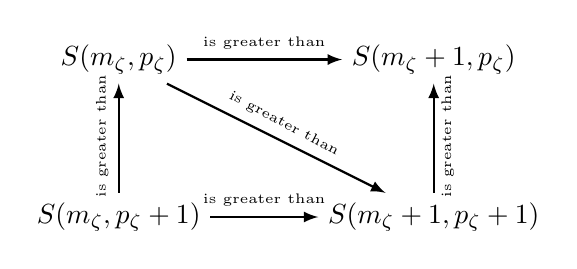
\begin{tikzpicture}
    \node[] (S00) at (0,0) {$S(m_\zeta,p_\zeta)$};
    \node[] (S10) at (4,0) {$S(m_\zeta+1,p_\zeta)$};
    \node[] (S01)  at (0,-2) {$S(m_\zeta,p_\zeta+1)$};
    \node[] (S11)  at (4,-2) {$S(m_\zeta+1,p_\zeta+1)$};
    \draw[->,thick,>=latex] (S00) -- node[anchor=south] {\tiny{is greater than}} (S10);
    \draw[->,thick,>=latex] (S01) -- node[anchor=south] {\tiny{is greater than}} (S11);
    \draw[->,thick,>=latex] (S11) -- node[anchor=west,xshift=5,yshift=-25,rotate=90] {\tiny{is greater than}} (S10);
    \draw[->, thick,>=latex] (S00) -- node[anchor=south,rotate=-28] {\tiny{is greater than}} (S11);
    \draw[->,thick,>=latex] (S01) -- node[anchor=west,xshift=-6,yshift=-25,rotate=90] {\tiny{is greater than}} (S00);
\end{tikzpicture}
\caption{Behaviour of the landscape of Surprise $S$.}
\label{fig:surprisebehaviour}
\end{figure}

A fourth inequality $S(m_\zeta,p_\zeta+1)>S(m_\zeta+1,p_\zeta)$ is implicit by looking at the behaviour of $S(\zeta)$ for a given graph. 
%\subsection{Pareto optimality}
The scheme in Figure~\ref{fig:surprisebehaviour} allows to rank the values of Surprise in relation to changes in $m_\zeta$ and $p_\zeta$. It's easy  verify that $S$ satisfies the following strict order relation:
\begin{equation}\label{eq:surpriseorderrelation}
S(m_\zeta+1,p_\zeta)<S(m_\zeta+1,p_\zeta+1)<S(m_\zeta,p_\zeta)<S(m_\zeta,p_\zeta+1).
\end{equation}
This property leads us to the observation that Surprise $S$ is a monotonically decreasing function (increasing $\hat{S}$) of $m_\zeta$ and monotonically increasing function (decreasing $\hat{S}$) of $p_\zeta$ in the convex interval $\mathcal{L}$.
Moreover, from Figure~\ref{fig:surprisebehaviour} follows that optimal solutions with respect to $S$ are Pareto-optimal with respect to maximizing $m_\zeta$ and minimizing $p_\zeta$.
In other words, a partition that is optimum with respect to Surprise is such that no further increment in $m_\zeta$ leads to a decrement in $p_\zeta$ that has higher $\hat{S}$.
The Pareto optimality of optimum Surprise partitions, implies that a perturbation of $\delta m_\zeta, \delta p_\zeta$ leads to a change in Surprise such that it monotonically decreases if and only if $\delta m_\zeta > \delta p_\zeta$, precisely:
\begin{equation}\label{eq:resolution_limit_condition}
S(m_\zeta + \delta_{m_\zeta}, p_\zeta + \delta_{p_\zeta}) < S(m_\zeta,p_\zeta) \iff \delta_{m_\zeta} \geq \delta_{p_\zeta}.
\end{equation}

%% \begin{figure}[htb!]
%% \centering
%% \begin{tikzpicture}[scale=0.8, every node/.style={scale=0.8}]
%% \def \S {1};
%% \def \W {11};
%% \def \H {7};
%% \node[anchor=south west, inner sep=0mm] at (0,0) { 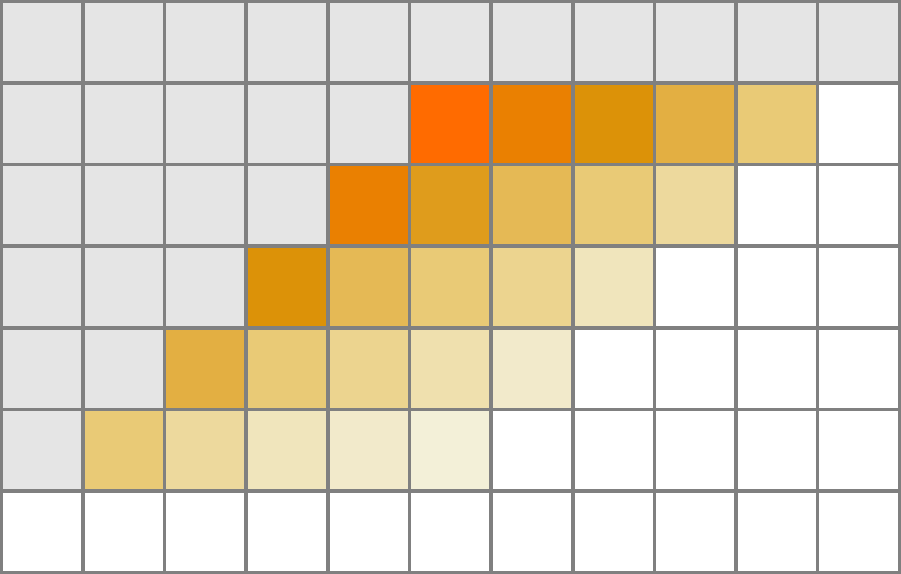
\includegraphics[width=\W cm]{images/plot_surprise_pareto.pdf}};
%% \node[anchor=south] at (\W /2,\H +0.25) {$\hat{S}=-\log_{10}(S(m_\zeta,p_\zeta$, $m=10$,$p=15$))};
%% %\draw[help lines,xstep=1.0,ystep=1.0] (0,0) grid (\W,\H);
%% \foreach \x in {1,...,\W } {\node [anchor=north] at (\x-0.5,0) {$\x$}; }
%% \node[anchor=north] at (\W/2,-0.5){$p_\zeta$};
%% \foreach \y in {1,...,\H} {\node [anchor=east] at (0 ,\y-0.5) {$\y$}; }
%% \node[anchor=east] at (-0.5,\H/2){$m_\zeta$};
%% %\node[rectangle,fill=black!10,draw=black,rounded corners=0.1cm] at (\W+1.5,\H-0.5) {$m_{\zeta},p_\zeta \not \subset \mathcal{L}$};
%% \end{tikzpicture}
%% \caption{Pareto optimality of Surprise (here $\hat{S}$ is represented) on a trivial graph with $n=6$ nodes and $m=7$ edges. No increment in $m_\zeta$ leads to a decrement in $p_\zeta$ that has higher $\hat{S}$. Here Surprise is optimal for $m_\zeta=6,p_\zeta=6$.}
%% \label{fig:pareto_optimality_surprise}
%% \end{figure}
%% \todo[inline]{CONTROLLARE FIGURA PROBABILMENTE SBAGLIATA PERCHE MZETA>M!!!}

The result in Eq.\ref{eq:resolution_limit_condition} is of great help in designing optimization algorithms as every move that increase the intracluster edges more than intracluster pairs is good, while moves that increase intracluster pairs more than intracluster edges must be ignored, therefore sparing time for the computation of Surprise. Additionally, Eq.~\ref{eq:resolution_limit_condition} is useful when analyzing the onset of the resolution limit for different models.
In the next sections we will show to what extent Surprise is affected by the resolution limit for Surprise, to show with convincing theoretical arguments that $S$ is nearly resolution-limit-free in Traag's sense~\cite{traag2015}.

%%%%%%%%%%%%%%%%%%%%%%%%%%%%%%%%%%%%%%%%%%%%%%%%%%%%%%%%%%%%%%
%%%%%%%%%%%%%%%%%%%%%%%%%%%%%%%%%%%%%%%%%%%%%%%%%%%%%%%%%%%%%%
%%%%%%%%%%%%%%%%%%%%%%%%%%%%%%%%%%%%%%%%%%%%%%%%%%%%%%%%%%%%%%
\subsection{Surprise is a statistical test}\label{sec:surprisefishertest}
Surprise considers the problem of community detection as the one of making the intracluster density as further as possible from the global density in statistical terms. In this sense, it's worth noting that $S$ is \emph{p}-value of a one-tailed Fisher exact-test where one is asking how confidently should reject the null hypothesis $H_0$ that the intracluster density is the same as the graph density.
It turns indeed out that this problem has an equivalent description in statistics, where one seeks to maximize the \emph{odds-ratio} of the $2 \times 2$ contingency table defined in Table~\ref{tab:contingency_table}.

The Fisher exact test implemented by Surprise is, as its name states, exact as long as the contingency table keeps the row and column totals fixed, and it can therefore be used regardless of the sample characteristics. A simpler $\chi^2$ statistic can be used when the elements of the contingency table are large enough, although only an approximation of the \emph{p}-value can be obtained.
In this case it's possible to tackle the problem of computation of $S$ by means of odds-ratio. Precisely, the \emph{normalized log odds-ratio} is computed as 
\begin{equation}
\log(\textrm{OR}) = \log\left( \frac{m_\zeta(p-m-p_\zeta+m_\zeta)}{(m-m_\zeta)(p_\zeta-m_\zeta)} \right )
\end{equation}
and in the asymptotic case, Surprise is equal to the probability:
\begin{equation}\label{eq:prob_or_se}
\Pr\left(z < -\frac{|\log\textrm{OR})|}{SE} \right)
\end{equation}
where $z$ is a random variable with standard normal distribution $z \approx \mathcal{N}(0,1)$.
Although not interesting in the case of binary graphs, equation~\ref{eq:prob_or_se} is telling us that in developing a version of Surprise that will keep into account weighted graphs, we should in some way rely on its asymptotic distribution.

\begin{table}[htb!]
\centering
\begin{tabular}{|c|c|c|c|}
\hline
 & Drawn & Not drawn & \textbf{Total}\\
\hline
Intracluster & $m_\zeta$ & $p_\zeta-m_\zeta$ & $p_\zeta$\\
\hline
Intercluster & $m-m_\zeta$ & $p-m-p_\zeta+m_\zeta$ & $p-p_\zeta$ \\
\hline
\textbf{Total} & $m$ & $p-m$ & $p$ \\
\hline
\end{tabular}
\caption{Contingency table for the urn model.}
\label{tab:contingency_table}
\end{table}

%%%%%%%%%%%%%%%%%%%%%%%%%%%%%%%%%%%%%%%%%%%%%%%%%%%%%%%%%%%%%%
%%%%%%%%%%%%%%%%%%%%%%%%%%%%%%%%%%%%%%%%%%%%%%%%%%%%%%%%%%%%%%
%%%%%%%%%%%%%%%%%%%%%%%%%%%%%%%%%%%%%%%%%%%%%%%%%%%%%%%%%%%%%%
\section{Resolution limit and Surprise}
Unfortunately, the resolution limit appears to be an intrinsic feature of many quality functions, and there appears to be a ``narrow scope to resolution-limit-free methods''~\cite{traag2015}.  
Surprise has been shown to outperform other network partitioning methods in the detection of small features within large graphs, but the extent to which it suffered from the resolution limit was unknown~\cite{aldecoa2011,aldecoa2013}, until our work~\cite{nicolini2016}.

As pointed out by Aldecoa~\cite{aldecoa2011}, the author who originally introduced Surprise, while Modularity-based methods define a community as a region with an unexpectedly high density of links with respect to the global characteristics of the network, Surprise weights the number of actual intracluster edges against the maximum number of links given the nodes in the clusters.
Hence, Surprise is able to discriminate local subnetworks whose internal density is close to that of a clique independently of their size.
In the following, we assess the extent to which the resolution limit may affect Surprise.

In order to assess to what extent Surprise is affected by the resolution limit, we directly compared Newman's Modularity and Surprise in the example of Fortunato and Barthelemy as illustrated in the previous chapter in Figure~\ref{fig:figure_1_barthelemy}. Already for $m_{12} = 1$, i.e. when the two cliques $G_1$ and $G_2$ were connected by only one edge, $Q^N$ showed sign inversion for $m_0 \approx 200$, meaning that it was beneficial for Modularity to merge two cliques.
In this same example though, Surprise instead never merges cliques, as made evident in Figure~\ref{fig:barthelemy_surprise}.

\begin{figure}[htb!]
\centering
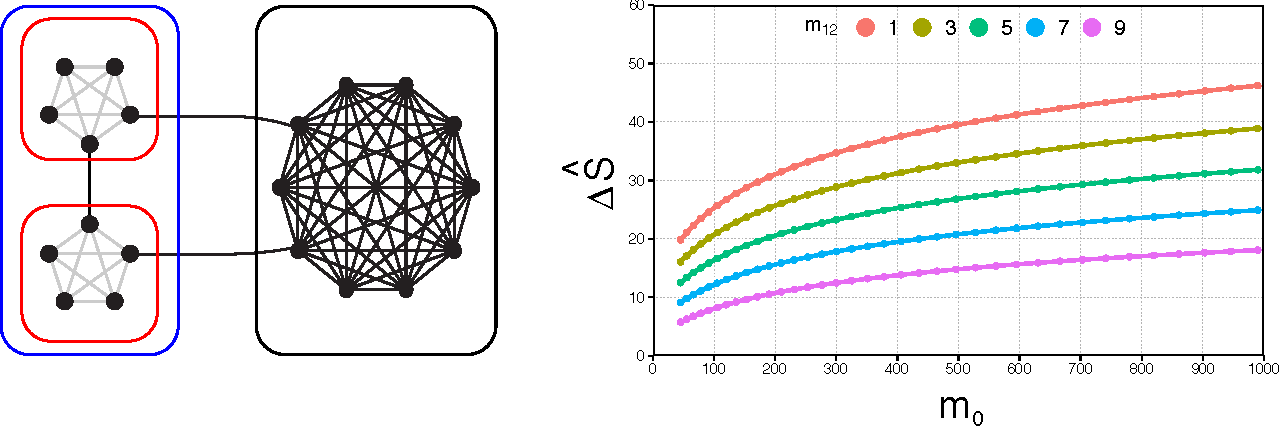
\includegraphics[width=1.0\textwidth]{images/barthelemy_surprise.pdf}
\caption{Difference in $\hat{S}$ between the partition where the two cliques are separated (red) and the partition where the two cliques are merged (blue), as in the benchmark network of Fortunato and Barthelemy. As the quantity $\Delta \hat{S}$ is always positive, Surprise is never going to merge cliques, independently from other global parameters. Adapted from Nicolini and Bifone~\cite{nicolini2016}.}
\label{fig:barthelemy_surprise}
\end{figure}

Figure~\ref{fig:barthelemy_surprise} shows that Surprise does not suffer from the resolution limit at least in this specific case.
Indeed, $\Delta \hat{S}$ was always positive and grew monotonically with increasing $m_0$. 
Hence, the two cliques $G_1$ and $G_2$ were always resolved by Surprise as separate communities independently of the network size, and also in the presence of some ``fuzziness'', i.e. when $m_{12}>1$ and the two cliques were connected by more than one edge.
In order to assess whether this behavior reflects a general property of Surprise, or is incidental to this particular example, we have also studied a generalization of Fortunato and Barthelemy's model.

A consequence of the definition of a resolution limit free in Traag's sense, is that such method will never depend on the size of the network to merge cliques in a graph comprising $r$ cliques of $n_r$ nodes connected in a ring structure as in Figure~\ref{fig:traag_ring_of_cliques} (often called the ``ring of cliques'' model).
This observation prompted us to explore the behavior of $\hat{S}$ in the ring of cliques model graph, as an extension of Fortunato and Barthelemy's model.
Interestingly, given its two-variables formulation, Surprise optimization can be seen as a multiobjective optimization problem where one seeks to minimize the intracluster pairs while maximizing the number of intracluster edges.
With increasing graph size, the computational problem of calculating $\hat{S}$ for every possible partition becomes rapidly intractable (maximization of $S$ is NP hard)~\cite{fleck2014}.
However, as explained before and pointed out by Fleck et al.~\cite{fleck2014}, the Surprise optimal clustering must be Pareto optimal with respect to minimizing $p_\zeta$ and maximizing $m_\zeta$, i.e. any further improvement in one of the two variables must occur at the expense of the other.

In this sense, the problem of Surprise optimization is shown to be equivalent to a linear program~\cite{fleck2014}, where one seeks to minimize $p_\zeta$ while keeping $m_\zeta$ equal to a constant $h$ from $1$ to $m$, choosing then among the resulting $m$ clusterings, the one that maximizes $\hat{S}$.
Hence, to delineate the Pareto frontier in the $(m_\zeta,p_\zeta)$ space, we need to solve $m$ integer linear programs (ILP) in the form:
\begin{align}\label{eq:surprise_ilp}
\textrm{minimize} \sum_{\{i,j\} \in \binom{V}{2}} \mathcal{X}_{ij} \nonumber \\
\textrm{s.t.} \quad \mathcal{X}_{ij} \in \{0,1 \} \nonumber \\
\quad \mathcal{X}_{ik} + \mathcal{X}_{ki} - \mathcal{X}_{ij} \leq 1 \nonumber \\
\sum_{\{i,j\} \in E} \mathcal{X}_{ij}=h \nonumber
\end{align}
where $\mathcal{X}_{ij}$, equivalent to $\delta(\sigma_i, \sigma_j)$, are a set of $\binom{n}{2}$ binary variables corresponding to vertex pairs, with the interpretation that $\mathcal{X}_{ij}=1$ if vertex $i$ and vertex $j$ are in the same community. The alternative objective function $\sum_{ij}\mathcal{X}_{ij}$ measures the number of intracluster pairs $p_\zeta$, while the number of intracluster edges $m_\zeta=\sum_{ij \in E} \mathcal{X}_{ij}$ was set equal to a fixed $h \in [0,m]$. The remaining constraints are necessary in order to ensure transitivity, i.e. if nodes $i$ and $j$ are in the same community, nodes $i$ and $k$ are in the same community, then nodes $j$ and $k$ share the same community too. 
Figure~\ref{fig:ring_cliques_pareto} shows the Pareto frontier for a ring of cliques where we independently varied the number of cliques $r$ and the number of nodes $n$ in every clique\footnote{Linear programs were solved using the Python interfaces of Gurobi 5.7.3 on Linux (Gurobi Optimizer Version 5.7, Gurobi Optimization, Inc., Houston, Texas, United States).}.
As $\hat{S}$ reaches its minimum (zero) both in the case where all nodes are separated communities ($p_\zeta=0$) or when a single community entails all nodes ($p_\zeta=p$), Figure~\ref{fig:ring_cliques_surprise} shows monotonically increasing Surprise along the frontier with increasing $p_\zeta$ up to the Surprise optimum, indicated by black circles in the Pareto front of Figure~\ref{fig:ring_cliques_pareto}, whereas the corresponding partition identified each clique as a separate community.
Importantly, in the range of parameters we have investigated, Surprise optimization never merged cliques in the ring of cliques, independently of the size of the graph, and behaved as a Traag's resolution-limit free method.

\begin{figure}[htb!]
\centering
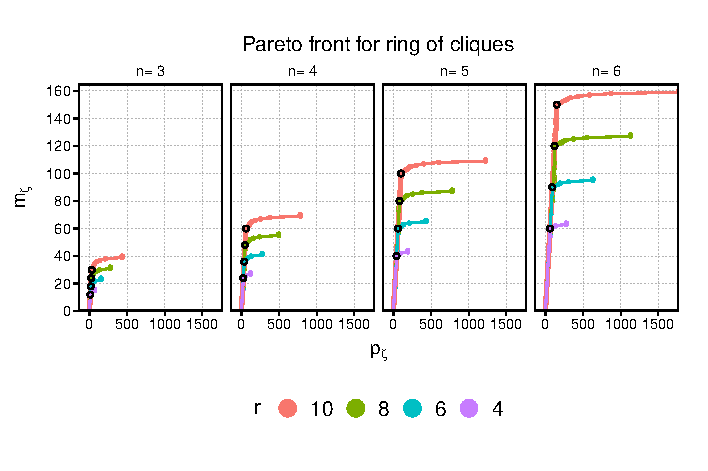
\includegraphics[width=0.8\textwidth]{images/ring_cliques_pareto.pdf}
\caption{Pareto front for a ring of cliques graph. Optimal solutions with respect to Surprise are indicated as small black dots. Adapted from Nicolini and Bifone~\cite{nicolini2016}.}
\label{fig:ring_cliques_pareto}
\end{figure}

\begin{figure}[htb!]
\centering
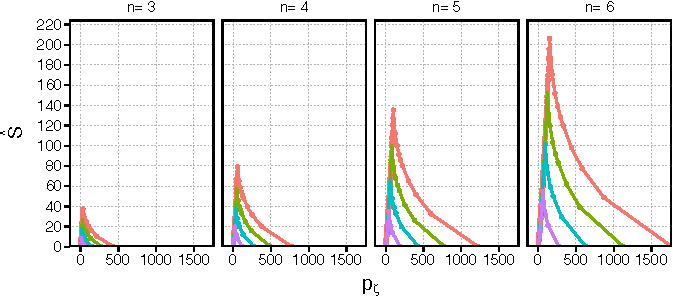
\includegraphics[width=0.8\textwidth]{images/ring_cliques_surprise.pdf}
\caption{Surprise $\hat{S}$ for a ring of cliques graph at different levels of $p_\zeta$ for corresponding solutions at fixed $m_\zeta$. The peak of $\hat{S} $is always reached at $p_\zeta$ when the modules entail single cliques separately. Adapted from Nicolini and Bifone~\cite{nicolini2016}.}
\label{fig:ring_cliques_surprise}
\end{figure}

While it is likely that this property is quite general and can be extended to every ring of cliques, an analytical demonstration is hampered by the non-additivity of the Surprise function.
Nonetheless, the size of the graphs we have explored numerically is quite typical of brain-connectivity networks and we feel encouraged to apply Surprise maximization to the study of the community structure of the brain.

Curiously, the maximum value of Surprise for given $(m_\zeta,p_\zeta)$ is sharply peaked and very different from other partitions, indicating that at least in this case Surprise shows no degeneracy of optimal solutions, as instead shown for Modularity in Section~\ref{sec:degeneracy}.
This observation led us to investigate to what extent Surprise is affected by the degeneracy problem.
We repeated the procedure indicated in section~\ref{sec:degeneracy}, where we embedded the complex landscape of partitions in a three dimensional space in order to show whether optimal Surprise solutions group in a large plateau of high Surprise values or not. As previously introduced, the global optimum is a sharply distinct partition, sitting on top of the embedded manifold, as illustrated in Figure~\ref{fig:degeneracy_surprise}.

\begin{figure}[ht]
\centering
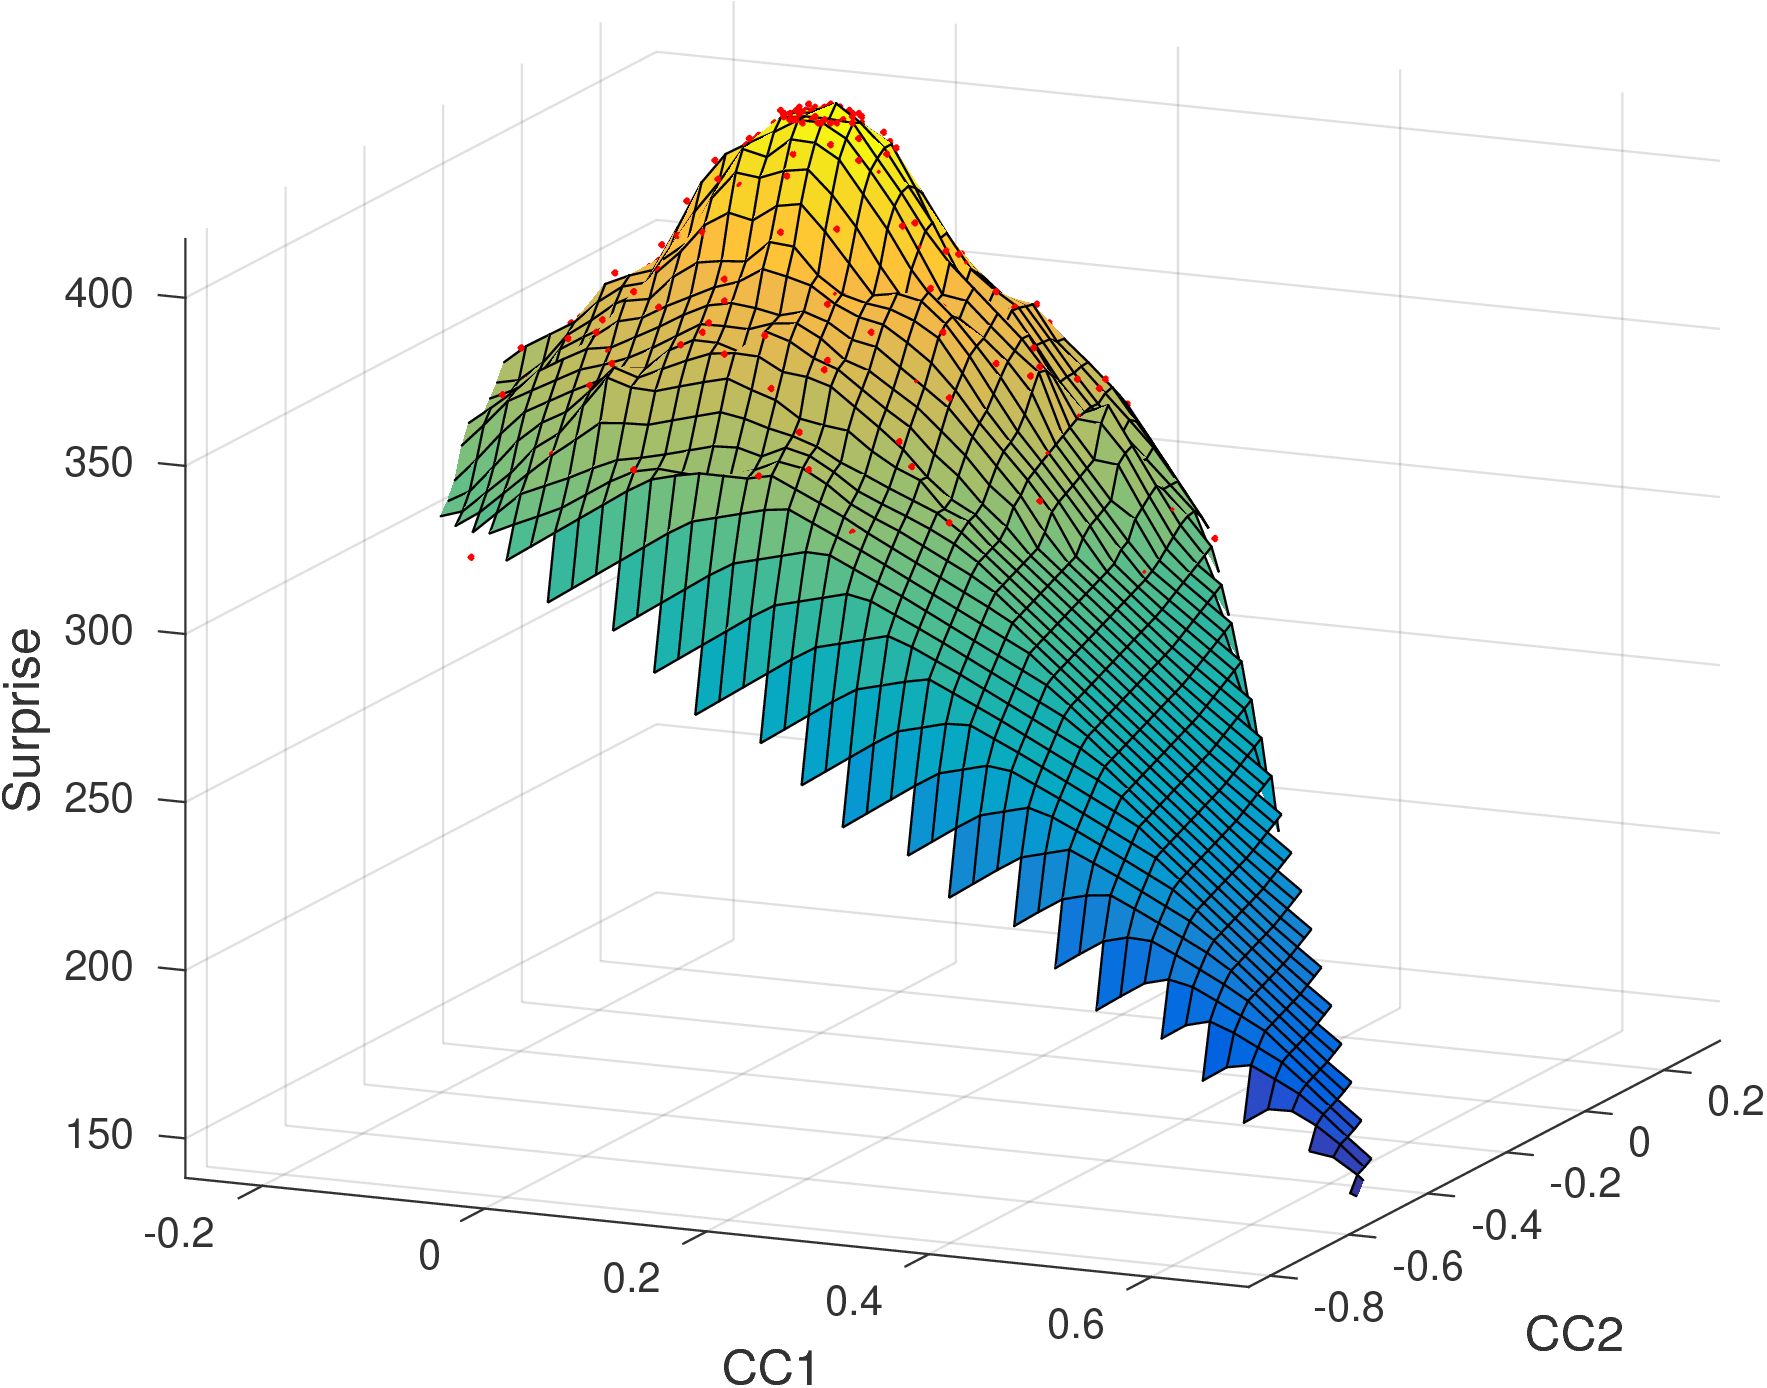
\includegraphics[height=0.4\textwidth]{images/degeneracy_surprise_n_5_c_24.png}\hfill
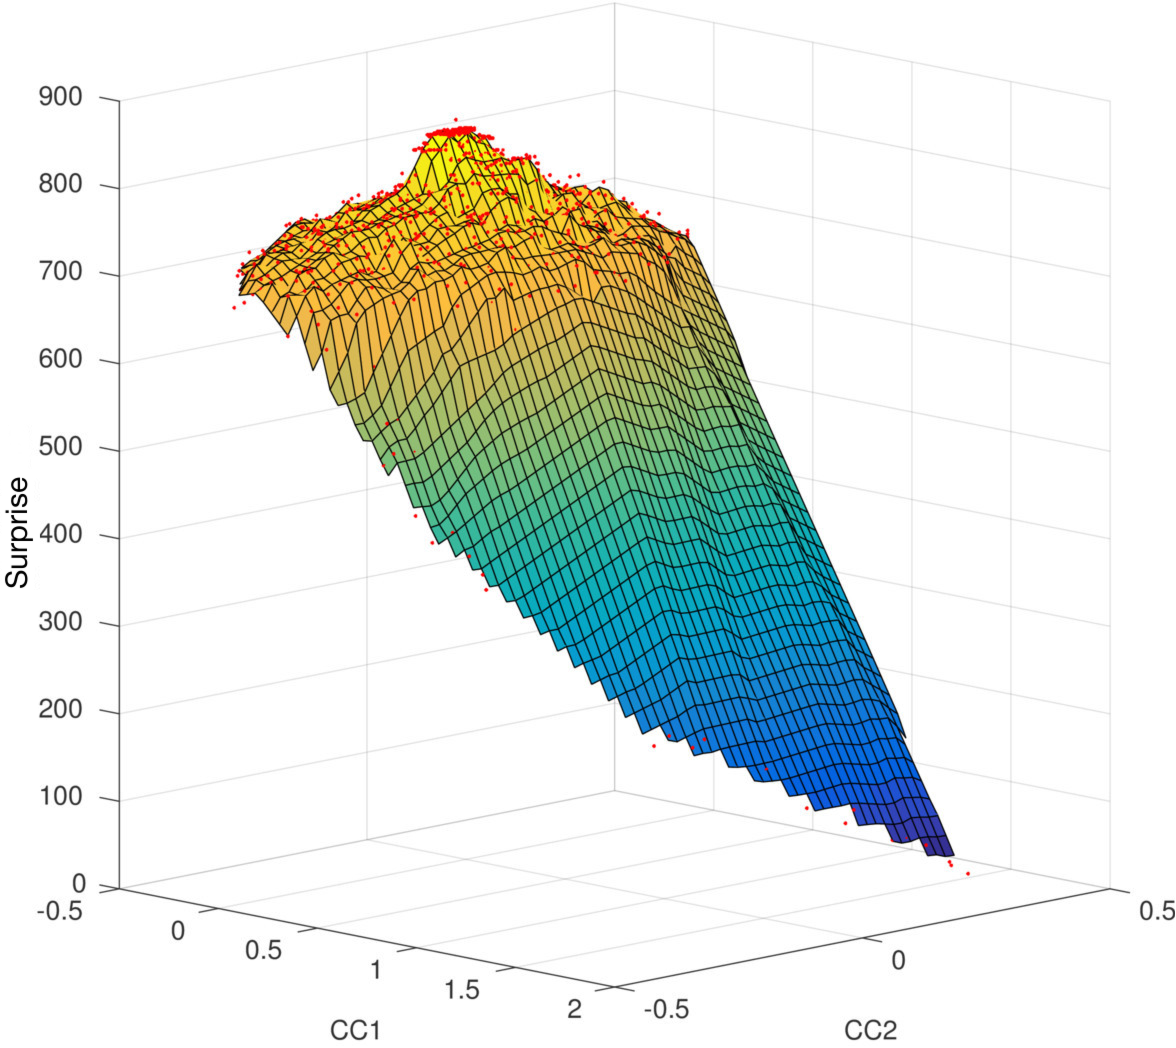
\includegraphics[height=0.4\textwidth]{images/degeneracy_surprise_n6_c30.png}
\caption{Degeneracy of Surprise landscape in a small (left) and large (right) ring of cliques graph. No plateaus exist, indicating the uniqueness of the global maximum that emerges from the other local optima.}
\label{fig:degeneracy_surprise}
\end{figure}

%%%%%%%%%%%%%%%%%%%%%%%%%%%%%%%%%%%%%%%%%%%%%%%%%%%%%%%%%%%%
%%%%%%%%%%%%%%%%%%%%%%%%%%%%%%%%%%%%%%%%%%%%%%%%%%%%%%%%%%%%
%%%%%%%%%%%%%%%%%%%%%%%%%%%%%%%%%%%%%%%%%%%%%%%%%%%%%%%%%%%%


\section{Maximization of Surprise: FAGSO}\label{sec:max_surprise_fagso}

Community detection is a NP-hard problem, and heuristics have to be developed for the optimization of quality functions for relatively large networks. In their original paper, Aldecoa et al.~\cite{aldecoa2011} applied metaheuristics, involving the evaluation of Surprise for partitions resulting from seven different community detection methods, each of those maximizing different quality functions.
Here, we describe direct maximization of Surprise by exploiting FAGSO~\cite{jiang2014}, an agglomerative optimization algorithm that builds on a variation of the Kruskal algorithm for minimum spanning tree~\cite{leiserson2001}.
The detailed pseudocode of this algorithm is reported in Algorithm~\ref{alg:fagso} and illustrated step by step on an example network in Figure~\ref{fig:fagso_working}.

The first step of FAGSO consists in ranking the edges in the graph in decreasing order by the Jaccard index of the neighbors of their two endpoints nodes.
An union-find data structure is used to hold the community structure throughout the computation.
At the beginning, each community consists only of one vertex.
Then, starting from the edge with the highest Jaccard index at the top of the list, the endpoints are attributed to the same community by disjoint-set union if this operation leads to a strictly better Surprise and if they do not belong already in the same community.
This step is repeated for all edges and the final community structure is returned in the disjoint-set.
FAGSO finds partitions with high Surprise and it is deterministic, unless two edges with the same Jaccard index are found. In this case, ties are broken at random. 

The implementation of FAGSO in \texttt{C++}, \texttt{Python} and \texttt{GNU Octave} is freely available at \url{https://github.com/carlonicolini/fagso}.

\begin{Algorithm}[htb!]
%%%% FAGSO %%%%
\begin{small}
\begin{codebox}
\Procname{$\proc{Fagso}(G)$}
\li $S\gets 0$ \Comment \emph{Initialize Surprise to $0$}
\li $D \gets \emptyset$ \Comment \emph{Initialize disjoint set forest}
\li \For each vertex $v$ in $V[G]$
\li \Do \proc{Make-Set}(v)
\End
\li $E' \gets \proc{Sort-Jaccard}(E)$ \Comment \emph{Sort edges in decreasing order by Jaccard index}
\li \For each edge$(u,v) \in E'$, \Comment \emph{Taken in decreasing order by Jaccard index}
\li \Do \If $\proc{Find-Set}(u) \neq \proc{Find-Set}(v)$
\li \Then \If $\proc{Surprise}(G,D \cup \{ (u,v)\} ) > S$
\li $D \gets D \cup  \{(u,v)\}$
\li $\proc{Union(u,v)}$ \Comment\emph{Merge the communities $u$ and $v$ belong}
\li $S=\proc{Surprise}(G,D)$ \Comment \emph{Update current Surprise}
\End
\End
\li
\Return $D$
\end{codebox}

%%%% MAKE-SET %%%%
\begin{codebox}
\Procname{$\proc{Make-Set}(x)$}
\li $p[x] \gets x$
\li $rank[x] \gets 0$
\end{codebox}
%%%% LINK %%%%
\begin{codebox}
\Procname{$\proc{Link}(x,y)$}
\li \If $rank[x]>rank[y]$
\li \Then $p[y]\gets x$
\li \Else $p[x]\gets y$
\li \If $rank[x] = rank[y]$
\li \Then $rank[y] \gets rank[y]+1$
\End
\End
\end{codebox}
%%%% UNION %%%%
\begin{codebox}
\Procname{$\proc{Union}(x,y)$}
\li \proc{Link}(\proc{Find-Set}$(x)$,\proc{Find-Set}$(y)$)
\end{codebox}
%%%% FIND-SET %%%%
\begin{codebox}
\Procname{$\proc{Find-Set}(x)$}
\li \If $x\neq p[x]$
\li \Then $p[x] \gets \proc{Find-Set}(p[x])$
\End
\li\Return $p[x]$
\end{codebox}
%%%% SURPRISE %%%%
\begin{codebox}
\Procname{$\proc{Surprise}(G,D)$}
\li $m_{\xi} \gets 0$ \Comment \emph{Number of intracluster edges}
\li $p_{\xi} \gets 0$ \Comment \emph{Number of intracluster pairs of vertices}
\li $m \gets |E[G]|$ \Comment \emph{Number of edges}
\li $p \gets \binom{\left| V[G]\right|}{2}$ \Comment \emph{Number of pairs of vertices}
\li \For each $g$ in $\proc{Connected-Components-Subgraphs}(D,G)$
\li \Do $m_{\xi} \gets m_{\xi} + \left|E[g]\right|$
\li $p_{\xi} \gets p_{\xi} + \binom{\left| V[g]\right|}{2}$
\End
\li \Return $-\log_{10}\left( \sum \limits_{i=m_\zeta}^m \dfrac{\binom{p_\xi}{i}\binom{p-p_{\xi}}{m-i}}{\binom{p}{m}} \right)$
\end{codebox}
%%%% MST PRIM %%%%
% \begin{codebox}
% \Procname{\proc{MST-Prim}$(G,w,r)$}
% \li \For each $u \in V[G]$
% \li \Do $key[u]\gets \infty$
% \li $\pi[u] \gets $ NIL \End
% \li $key[r] \gets 0$
% \li $Q \gets V[G]$
% \li \While $Q \neq \emptyset$ 
% \li \Do $u\gets \proc{Extract-Min}(Q)$
% \li \For each $v \in Adj[u]$ 
% \li \Do \If $v\in Q$ and $w(u,v) < key[v]$
% \li \Then $\pi[v]\gets u$
% \li $key[v]\gets w(u,v)$
% \End
% \End
% \End
% \End
% \End
% \end{codebox}
\end{small}
\caption{Pseudocode of FAGSO, with description of the implementation of union-find data structure.}
\label{alg:fagso}
\end{Algorithm}

\begin{figure}[htb!]
\centering
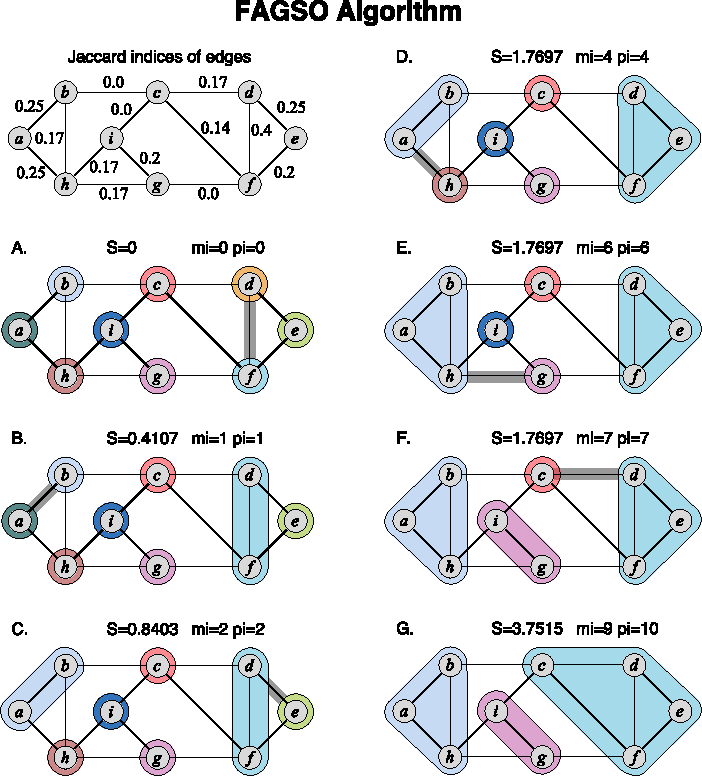
\includegraphics[width=0.8\textwidth]{images/fagso.pdf}
\caption{FAGSO algorithm steps illustrated. Firstly, Jaccard indices are computed. In box A., every node is associated to a separate community and FAGSO evaluates whether to merge nodes $d$ and $f$ in the same community as the edge they form has the highest Jaccard index. Since this merge results in an increased value of Surprise, $d$ and $f$ are merged in box B. then FAGSO proceeds to evaluate the merge of nodes $a$ and $b$ as their Jaccard index is the second greatest. FAGSO merges the two nodes in a second community and proceeds updating the Surprise value and analyzing the subsequent merges in boxes D to F, until no moves are available and FAGSO terminates with the community structure in box G.}
\label{fig:fagso_working}
\end{figure}

\subsection{Benchmarking FAGSO}


\section{From binary to weighted networks}
As described and illustrated in the previous chapter, a fundamental limitation of Surprise lies in its definition in terms of discrete probability and binomial coefficients that make it applicable only to binary networks, i.e. graphs with edge values $1$ or $0$.
This represents a substantial drawback, for it requires binarization of brain connectivity networks, thus discarding potentially important information contained in the edge weight distribution.
Moreover, different binarization procedures may lead to different network representations for the same connectivity dataset.
Therefore, an extension of Surprise to weighted networks would be highly desirable, and would provide a new and important tool to study the modular organization of brain connectivity beyond the resolution limit.


Capitalizing on recent development in the field of statistical physics of complex networks~\cite{traag2015}, we describe and demonstrate the use of Asymptotical Surprise, a weighted counterpart to Surprise, in the study of the modular structure of weighted networks.
Moreover, we propose a new algorithm, dubbed PACO (PArtitioning Cost Optimization) for the direct maximization of Asymptotical Surprise, that has its roots in the previously described FAGSO algorithm.

Since there is no ground-truth structure for brain functional connectivity networks, we have assessed the performance of this novel approach on synthetic networks with a planted modular structures, and compared it to some of the leading graph partitioning methods.
Importantly, we demonstrate our approach in networks  derived from synthetic data that mimic different structures, levels of noise and variability, such as those observed in functional connectivity experimental data.
Indeed, improved resolution afforded by Asymptotical Surprise may imply increased vulnerability to spurious modules resulting from noisy correlations.
It is therefore important to assess the benefits of increased resolution against the limitations arising from intrinsic data variability. 

Finally, we apply Asymptotical Surprise to weighted functional connectivity networks from resting state fMRI data, revealing a heterogeneous, multiscale community structure. We show that the finer modular subdivision of resting state functional connectivity networks obtained by Asymptotical Surprise leads to substantial differences in the identification of connector hubs compared to other community detection methods.

\section{Asymptotical Surprise}
As introduced in the previous sections, Surprise~\cite{aldecoa2011,aldecoa2013} is a quality measure of the partition of a binary network that has its roots in probability theory.
For a given partition $\zeta$, Surprise represents the probability that a graph drawn uniformly at random from the set of all graphs with $n$ nodes, $p=\binom{n}{2}$ pairs and $m$ edges has at least as many intra-cluster edges as $G$. Intuitively the lower the probability the better the partition.  For binary networks, Surprise can be computed within the discrete probability theory of urn models as shown in Equation~\ref{eq:surprise}.

In developing a quality function inspired to the principle of Surprise that works for weighted networks, it's convenient to consider the asymptotical expansion of the hypergeometric distribution. We introduce  $q=m_\zeta/m$ and $\left<q \right>=p_\zeta/p$ as the observed and expected fraction of intracluster edges. By only taking into account the dominant term of the sum in Eq.~\ref{eq:surprise} (the one with $i=m_\zeta$), after some manipulations we get an approximate expression for the logarithmic Surprise\footnote{If not specified, starting from here we use natural base logarithms.}:
\begin{equation}\label{eq:surprise_dominant}
\log(S) \approx \log \left( \frac{\binom{\left<q\right> p}{m_\zeta} \binom{(1-\left<q\right>)p}{m(1-q)}}{\binom{p}{m}} \right)
\end{equation}
which corresponds to the probability of observing exactly $m_\zeta$ internal links, given the clustering $\zeta$. As the denominator in Eq.\ref{eq:surprise_dominant} is independent of the partition, we ignore it, and thanks to the Stirling approximation of the binomial coefficients, which reads 
\begin{equation}
\log \binom{n}{k} \approx k \log \left( \frac{n}{k} \right)
\end{equation}
we can write the dominant term~\ref{eq:surprise_dominant} as:
\begin{equation}
\log(S) = - \log \left(\frac{m}{p}\right)^{-m} \left[ \left(\frac{\left< q\right>}{q}\right)^q \left(\frac{1-\left< q\right>}{1-q}\right)^{1-q} \right]^{m}
\end{equation}
The term $(m/p)^{-m}$ is independent of the partition so we can discard it. Hence, the asymptotic expansion of Surprise reads:
\begin{equation}
\log(S) = -m \left[ q \log \frac{\left<q\right>}{q} + (1-q)\log \frac{1-\left<q\right>}{1-q} \right]
\end{equation}
Interestingly, this last equation corresponds to the binary Kullback-Leibler divergence $m D_{KL}(q \| \left< q \right>)$, which is interpretable as the distance between the two probability distributions $q$ and $\left<q\right>$, or more precisely, as the information lost (in nats since we are using natural base logarithms) when we encode the distribution $q$ with the distribution $\left< q\right>$. 
Thus, in the limit of large networks, Surprise $\hat{S}$ can be approximated by a binomial distribution. This observation led to definition of Asymptotical Surprise $\mathcal{S}_a$~\cite{traag2015}:
\begin{equation}\label{eq:asymptoticalsurprise}
\mathcal{S}_a = m D_{\textrm{KL}}\left( q \| \left< q \right> \right)
\end{equation}
where the binary Kullback-Leibler divergence~\cite{kullback1951} is $$D_{\textrm{KL}}(x\|| y) = x \log \left(\frac{x}{y} \right) + (1-x)\log \left (\frac{1-x}{1-y} \right).$$

In the framework of information theory~\cite{cover2006}, Asymptotical Surprise represents the Kullback-Leibler divergence between the observed and expected fraction of intra-cluster edges; it encodes the information lost when the prior distribution $\left <q \right >$ is used to approximate the posterior distribution $q$. Kullback-Leibler divergence is a quasi-distance on probability distributions as it is always non-negative, non-symmetric and zero only when $q=\left< q \right>$, exactly like binary Surprise.

Asymptotical Surprise has a simpler formulation than binary Surprise as there are no binomial coefficients to evaluate and it has been shown to be resolution-limit-free in the limit of large networks~\cite{traag2015}. As a side effect of its definition in terms of information-theoretic quantity, Asymptotical Surprise transparently allows the extension of Surprise to weighted networks, when the intracluster density now consider edge weights.
This powerful property made Asymptotical Surprise suited for community detection in weighted networks and in particular to brain functional connectivity networks, seamlessly permitting to avoid the need of binarization procedures prior to the community detection, as shown in~\cite{nicolini2017}.

Given its information-theoretic formulation, Asymptotical Surprise cleary features \emph{convexity}, a property that is more difficult to assess for binary Surprise. Optimization of convex functions is typically simpler due to some regularities featured by such functions and the availability of practical algorithms. Furthermore a convex function warranties a landscape with a global optimum and no degeneracy, a property that is extremely important for community detection.

Yet, numerical evalaution of Asymptotical Surprise is much faster than binary Surprise, furthermore it approximates very well Surprise already for networks with more than 50 nodes, as shown in Figure~\ref{fig:asymptotical_surprise_comparison}.

\begin{figure}[htb!]
\centering
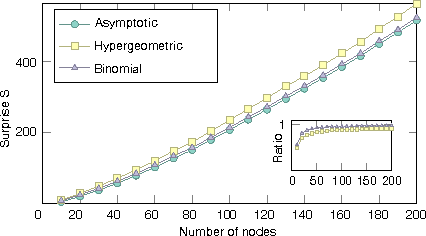
\includegraphics[width=1\textwidth]{images/asymptotical_surprise_comparison.pdf}
\caption{Approximation of binary Surprise with a binomial formulation and the Asymptotical formulation based on the Kullback-Leibler divergence. In the inset, the approximation ratio of binomial and Asymptotical Surprise to hypergeometric Surprise tends to 1 for graphs larger than 50 nodes. Adapted from~\cite{traag2015}.}
\label{fig:asymptotical_surprise_comparison}
\end{figure}


\subsection{Maximization of Asymptotical Surprise: PACO}
Finding the optimal partition of a graph is an NP-hard problem~\cite{fortunato2010} and practical implementations of community detection rely on heuristic approaches that enable finding nearly-optimal solutions in a reasonable computation time.

Here we introduce a powerful and general method for the optimization of Asymptotical Surprise dubbed PACO (PArtitioning Cost Optimization). PACO is a non-deterministic agglomerative algorithm based on FAGSO (described in chapter~\ref{sec:max_surprise_fagso}) and, like the Louvain method, has an element of randomness that enables a more efficient exploration of the partition landscape.

The operating principle of PACO is based on the triadic closure property, i.e. the fact that in real-world networks nodes with many common neighbors are more likely to be neighbors. This transitive neighborhood property underlies the formation of communities of nodes~\cite{bianconi2014,eustace2015}. In principle, any measure of structural similarity between nodes could guide a community detection heuristic toward the optimal partition. Specifically, PACO uses the Jaccard index~\cite{jaccard1901}, a measure of the fraction of overlap between the neighbors in common between nodes, as the guiding principle for the agglomeration of similar nodes in the same community.

In the first phase of PACO, the Jaccard metric is evaluated for every edge. More formally, for an edge $e=(u,v)$ the Jaccard index is computed as $J(e)=\frac{|\Gamma(u) \cap \Gamma(v)|}{|\Gamma(u) \cup \Gamma(v)|}$ where $\Gamma(u)$ and $\Gamma(v)$ are the neighboring nodes of $u$ and $v$ respectively.

The agglomerative process starts with an initial partition where every vertex represents a community on its own. This partition has $n$ communities and no intra-cluster edges.
The edges of the graph are then ranked in decreasing order by their Jaccard index and iteratively, for every edge in the sorted list, endpoint nodes are merged only if they belong to different communities. In this case one of the two endpoints, selected by chance, is assigned to the other's endpoint community and the increment of Surprise is computed: if it is positive, the partition is updated together with the new value of Surprise (or Asymptotical Surprise), otherwise the algorithm proceeds to the next edge.  

Figure~\ref{algo:paco} describes the details of the PACO algorithm for Surprise and Asymptotical Surprise Optimization.
The function \textsc{Paco} takes as input a graph G and returns the nodes community membership vector C. Line 1 initializes the value of Surprise to 0. Line 2 assign to each node in the graph its community. Line 3 creates a list of edges E' sorted in decreasing order by their Jaccard coefficient. Line 4 iterates on every edge e=(u,v) and at line 6 checks if the endpoints they share the same community. Line 8 copies the membership vector to a temporary vector C'. Lines 9-13 choose randomly at chance if to put node u in the community of v or viceversa. Line 14 computes the new value of Surprise S' from the just updated community membership C. The function \textsc{ComputeSurprise} returns the value of Surprise for graph G and partition C. Lines 15 to 18 checks if the new value of Surprise S' is greater than the previously stored value S and update Surprise and the membership vector, otherwise continue to the next edge. Line 19 returns the final community membership assignment.

%%%% PACO %%%%
\begin{Algorithm}[htb!]
\begin{codebox}
\Procname{$\proc{Paco}(G)$}
\li $S\gets 0$ \Comment \emph{Initialize Surprise to $0$}
\li $C \gets (1,\ldots,|V|)$  \Comment \emph{Initialize membership vector}

% \End
\li $E' \gets \proc{Sort-Jaccard}(E)$ \Comment \emph{Sort edges in decreasing order by Jaccard index}

\li \For each edge $(u,v)$ in $E'$
\li \Do \li \If $C[u] \neq C[v]$ \Comment \emph{try to move nodes only if in different communities}
\li \Then
\li $C' \gets C$ \Comment \emph{Create a temporary membership vector}
\li \If \proc{UnifRand(0,1)} $< 0.5$ 
\li \Then 
\li $C'[v] \gets C[u]$
\li	\Else
\li $C'[u] \gets C[v]$ \End
\li $S' =$ \proc{ComputeSurprise($G$,$C'$)}
\li \Do \If $S'>S$
\li \Then
\li $C \gets C'$ \Comment \emph{update membership}
\li $S' \gets S$ \Comment \emph{update Surprise}
\End
\End \End \End
\li \Return $C$
\end{codebox}
\caption{Pseudocode of the PACO algorithm.}
\label{algo:paco}
\end{Algorithm}

\subsection{Computational running time analysis}
We applied PACO on a full-resolution voxelwise connectivity matrix with 51,653 nodes and almost 2 million edges. PACO took 14 minutes for a single repetition on a server with Intel Xeon E5-2643@ 3.40 Ghz CPU and 256 GB ram.
We estimated that 2000 repetitions of PACO would take approximately 2.5 weeks on this server. We also tried to run PACO on a standard office PC with 16 GB memory and an Intel Core i7: it took almost 40 minutes. It’s important to notice that the running time of PACO is mainly determined by the computation of Jaccard indexes in the initial step.
The running time for this computation is in the order of $O(nd^2)$ where $n$ is the number of nodes and $d$ is the average degree of nodes. On a desktop workstation with a 2.5 GHz CPU, PACO runs in some tenths of seconds on a single repetition for a graph of around 600 nodes with a density close to 10\%, typical of brain networks. A small benchmark of PACO running times on a desktop workstation is shown in Figure~\ref{fig:paco_benchmark}, where we found optimal Surprise partitions of a LFR network with the parameters described in the text but increasing number of nodes.

\begin{figure}[htb!]
\centering
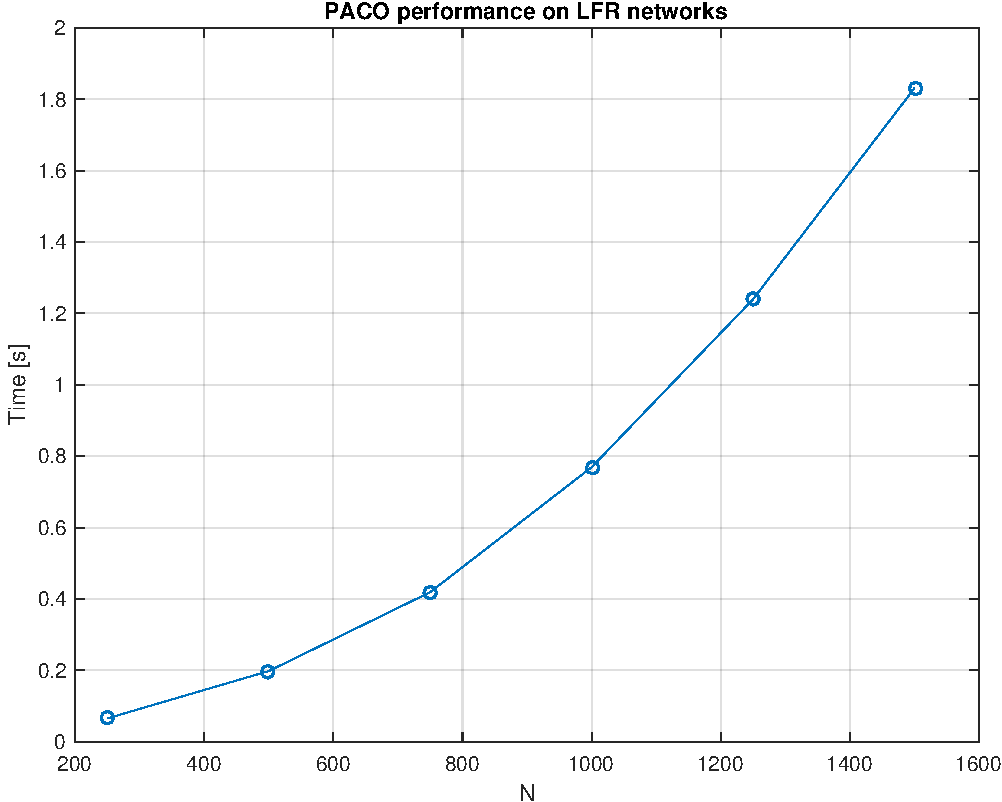
\includegraphics[width=0.5\textwidth]{images/paco_benchmark.pdf}
\caption{Performance of PACO on a LFR network with parameters}
\label{fig:paco_benchmark}
\end{figure}

\subsection{Best quality solution and number of repetitions}
In order to get a better idea of how fast the PACO method converges to a maximum, we have plotted the optimal value of Asymptotical Surprise over the 10000 runs for one instance of the LFR network, and for the resting state data-set presented in the Manuscript (Figures~\ref{fig:paco_variability_lfr},\ref{fig:paco_variability_bullmore}).
From these graphs, it appears that 2000 runs may be sufficient to reach stable community detection for the experimental data-set. A near-optimum value is reached earlier for the LFR network, but it should be noted that we have taken an instance of the synthetic network with no-noise added.

\begin{figure}[htb!]
\centering
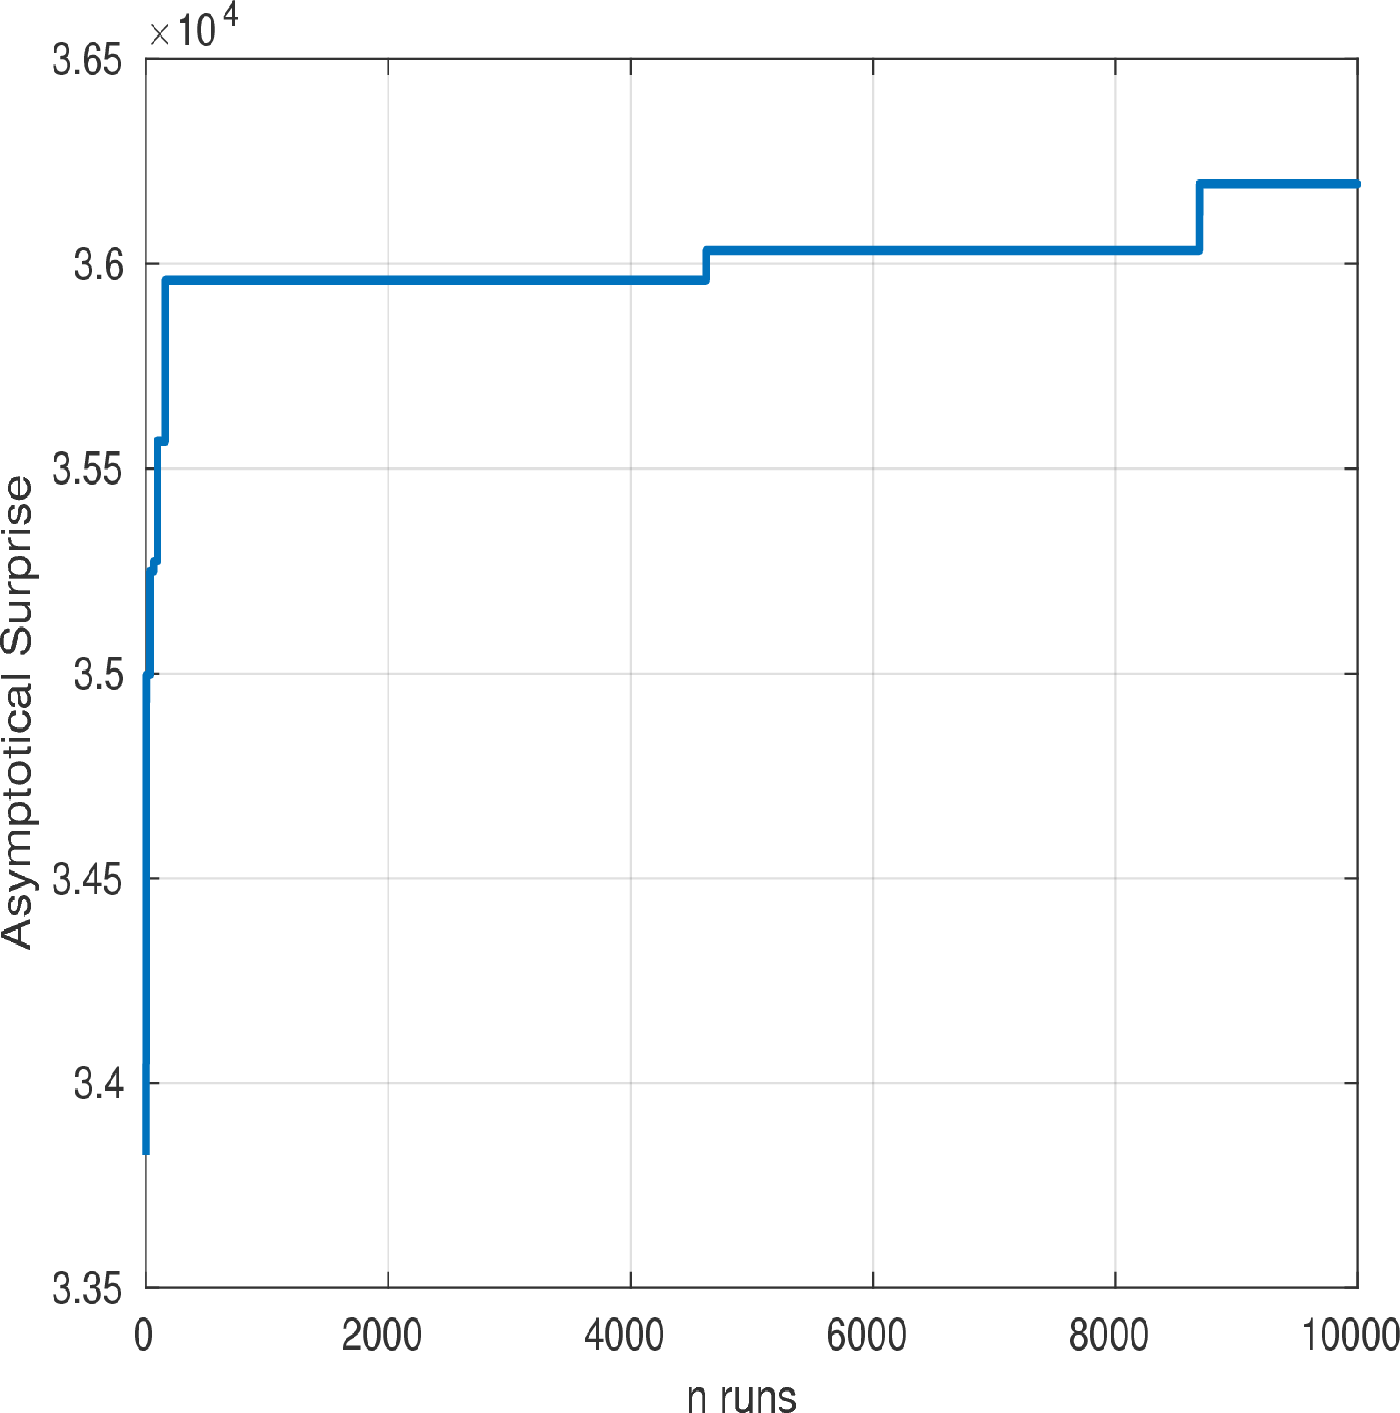
\includegraphics[width=0.5\textwidth]{images/paco_variability_nreps_lfr.png}
\caption{Maximum value of Asymptotical Surprise with respect to number of repetitions on a LFR networks as described in the main text.}
\label{fig:paco_variability_lfr}
\end{figure}
\begin{figure}[htb!]
\centering
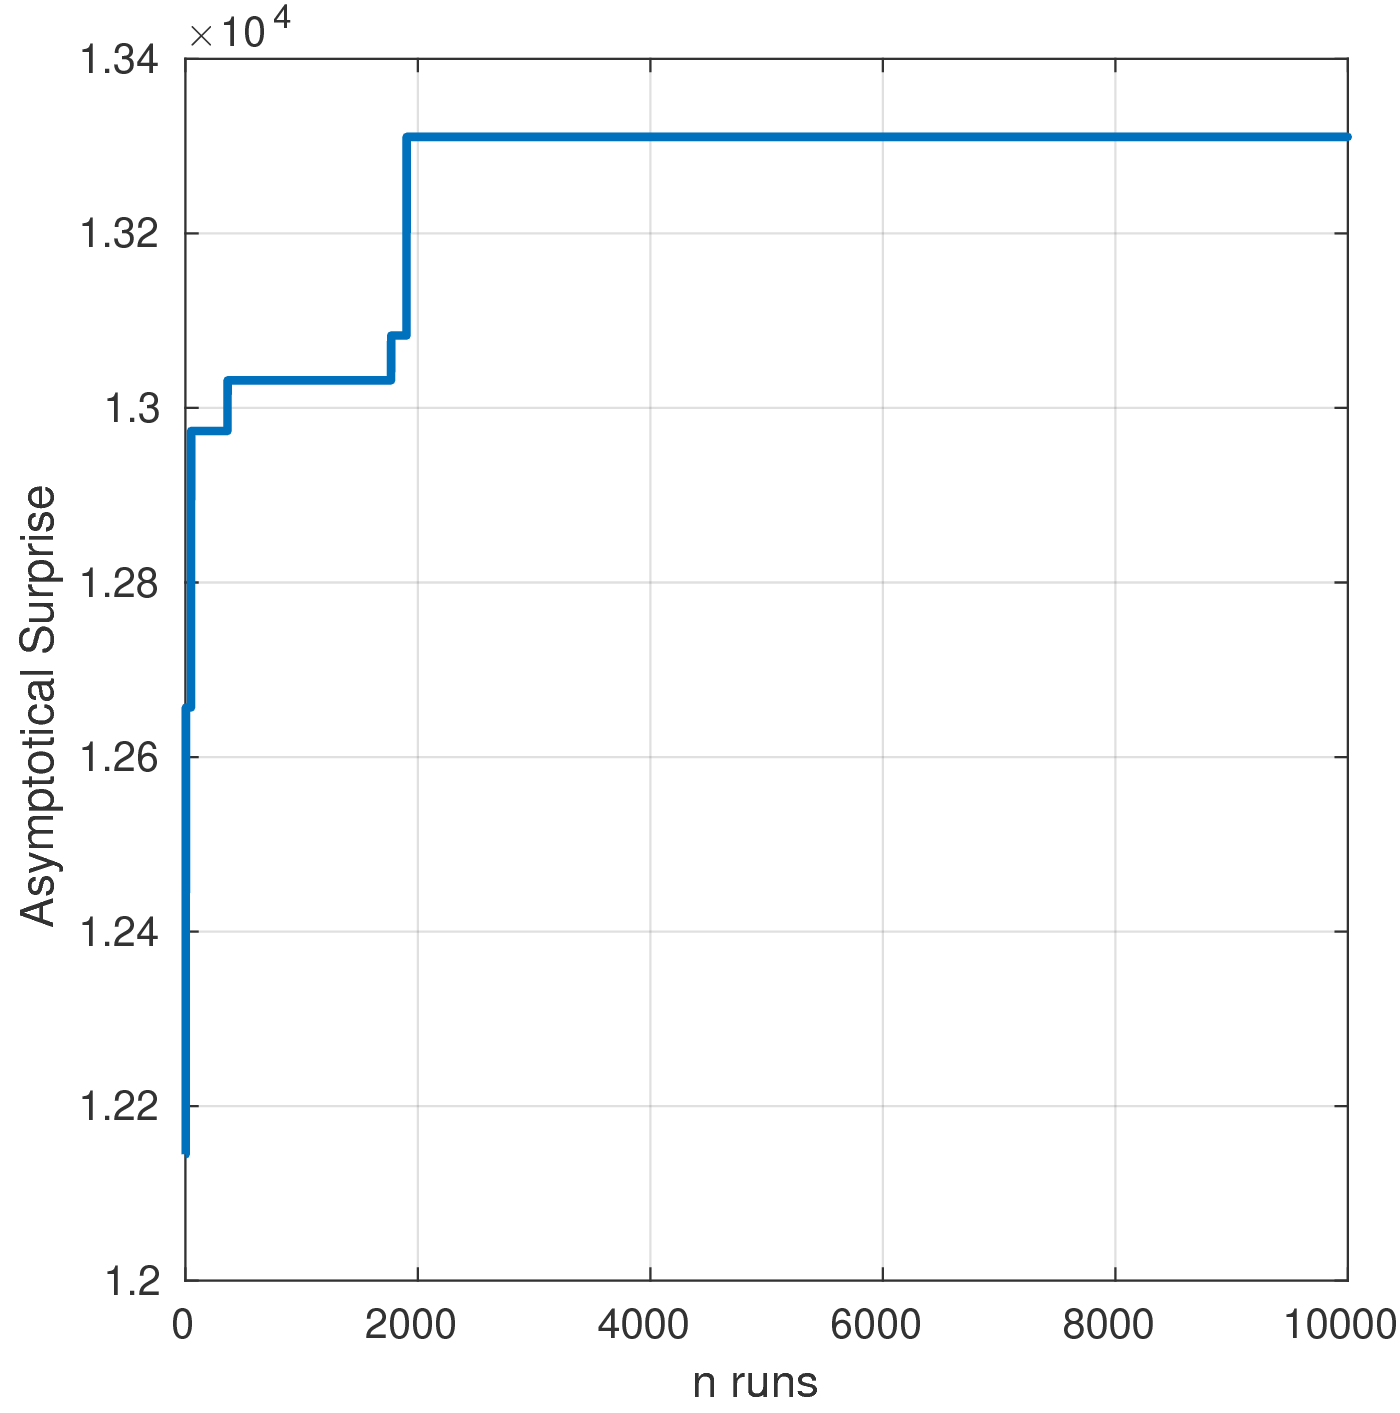
\includegraphics[width=0.5\textwidth]{images/paco_variability_nreps_bullmore.png}
\caption{Maximum value of Asymptotical Surprise with respect to number of repetitions on the resting state dataset described in the main text.}
\label{fig:paco_variability_bullmore}
\end{figure}

\subsection{Influence of LFR parameters on community detection performance}
Among the two most important parameters in the LFR benchmark are the topological and weights mixing coefficients. 
The topological mixing coefficient $\mu_t$ is the average ratio of intra-cluster neighbors divided by the number of inter-cluster neighbors, as defined in~\cite{lancichinetti2008}. The weights mixing coefficient is defined as the average ratio of node intra-cluster strength and inter-cluster strength, as defined in~\cite{lancichinetti2009a}.
We explored the effects of these parameters on the ability of PACO to retrieve the planted structure in the network.
We set $\mu_t=\mu_w$, as setting $\mu_w$ greater than $\mu_t$ would introduce inconsistency in the relative number and weight of the edges, with intermodule edges carrying the largest weights.

We analyzed the performance of Newman's Modularity, Infomap and PACO on LFR networks where we varied the topological and weights mixing coefficients.
In Figure~\ref{fig:avgmutmuw} the performance of the three methods is comparable in terms of NMI, with a faster decay of NMI for InfoMap and Newman compared to PACO for large $\mu_t$.

\begin{figure}[htb!]
\centering
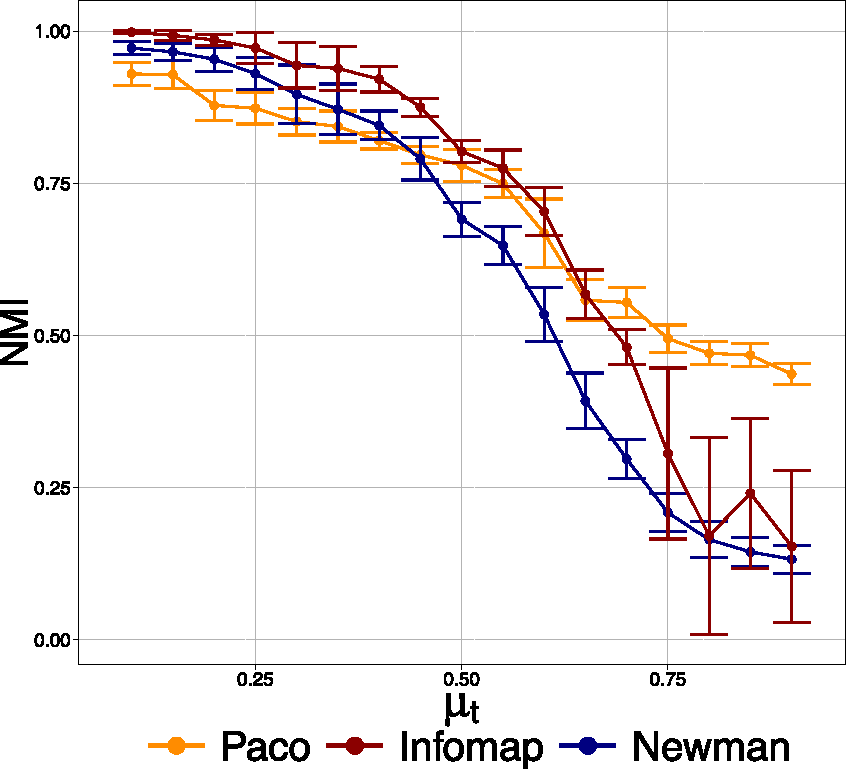
\includegraphics[width=0.5\textwidth]{images/avg_nmi_allmethods_lfr_errorbars.pdf}
\caption{NMI of the retreived vs planted partition of an LFR network as a function of $\mu_t=\mu_w$ for the three community detection methods}
\label{fig:avgmutmuw}
\end{figure}

\subsection{Comparison of PACO and FAGSO}

FAGSO is an agglomerative optimization algorithm that builds on a variation of the Kruskal algorithm for minimum spanning tree and is described in~\cite{nicolini2016}. The first step of this method consists in ranking the edges in the graph in decreasing order by the Jaccard index of the neighbors of their two endpoints vertices. An union-find data structure is used to hold the community structure throughout the computation. At the beginning, each community consists only of one vertex. Then, starting from the edge with the highest Jaccard index at the top of the list, the endpoints are attributed to the same community by disjoint-set union if this operation leads to a strictly better Surprise and if they do not belong already in the same community. This step is repeated for all edges and the final community structure is returned in the disjoint-set. This method finds partitions with high Surprise and it is deterministic, unless two edges with the same Jaccard index are found. In this case, ties are broken at random. 

PACO and FAGSO are based on the same idea of greedy agglomeration of edges that leads to increment in Surprise, but the implementation of the agglomeration step is different.
In the box A of Figure~\ref{fig:pacofagso} both the algorithms are considering whether to merge nodes from edge $d-g$ into the same community or not.
FAGSO consider the operation of merging nodes $d,g$ in the same community by joining red and blue communities together in one larger module and proceeds if this leads to higher Surprise.
PACO instead works at node level, considering whether to randomly move node $g$ in the red community (Box C) or node $d$ in the blue community (Box D). PACO chooses between the two options the one that leads to the highest increment in Surprise.
This detail allows PACO to explore more finely the landscape of optimization as it has more run to run variability. Additionally the internal implementation of PACO is faster as it stores the community structure as an array of integers representing the node affiliations, while FAGSO was storing the community structure as a set of nodes for every community.

\begin{figure}[htb!]
\centering
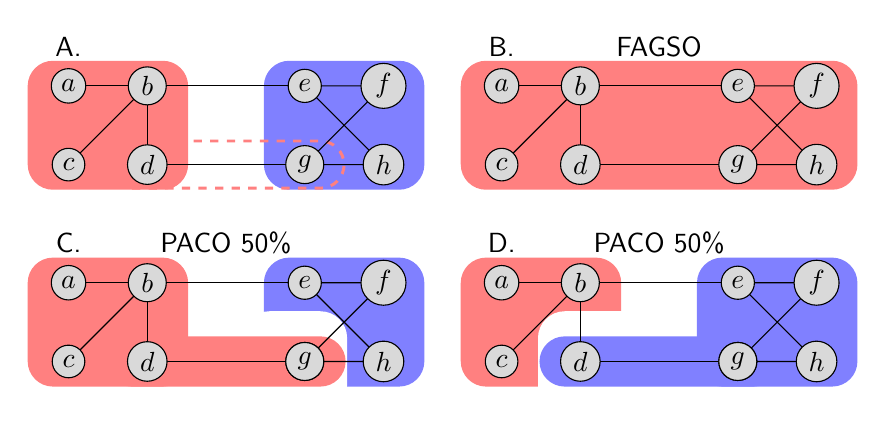
\begin{tikzpicture}
%\draw[help lines,step=1] (0,-5) grid (10,5);
\begin{scope}[shift={(0,0)}]
\fill [red!50, draw, rounded corners=2ex,line width=0.25ex] (-0.5,-0.3) rectangle (1.5,1.3);
\fill [blue!50, draw, rounded corners=2ex,line width=0.25ex] (2.5,-0.3) rectangle (4.5,1.3);
\draw [red!50, draw, rounded corners=2ex, dashed, line width=0.25ex] (0.5,-0.3) rectangle (3.5,0.3);
\draw (0,1) -- (1,1);
\draw (1,1) -- (1,0);
\draw (1,0) -- (1,1);
\draw (1,1) -- (0,0);
\draw (1,0) -- (3,0);
\draw (1,1) -- (3,1);
\node [fill=gray!30, radius=1ex, draw, circle, inner sep=2pt] at (0,1) {$a$};
\node [fill=gray!30, radius=1ex, draw, circle, inner sep=2pt] at (1,1) {$b$};
\node [fill=gray!30, radius=1ex, draw, circle, inner sep=2pt] at (0,0) {$c$};
\node [fill=gray!30, radius=1ex, draw, circle, inner sep=2pt] at (1,0) {$d$};
\draw (3,1) -- (4,1) -- (3,0) -- (4,0) -- cycle;
\node [fill=gray!30, radius=1ex, draw, circle, inner sep=2pt] at (3,1) {$e$};
\node [fill=gray!30, radius=1ex, draw, circle, inner sep=2pt] at (4,1) {$f$};
\node [fill=gray!30, radius=1ex, draw, circle, inner sep=2pt] at (3,0) {$g$};
\node [fill=gray!30, radius=1ex, draw, circle, inner sep=2pt] at (4,0) {$h$};
\node at (0,1.5) {\textsf{A.}};
\end{scope}

\begin{scope}[shift={(5.5,0)}]
\node at (2,1.5) {\textsf{FAGSO}};
\node at (0,1.5) {\textsf{B.}};
\fill [red!50, draw, rounded corners=2ex,line width=0.25ex] (-0.5,-0.3) rectangle (4.5,1.3);
\draw (0,1) -- (1,1);
\draw (1,1) -- (1,0);
\draw (1,0) -- (1,1);
\draw (1,1) -- (0,0);
\draw (1,0) -- (3,0);
\draw (1,1) -- (3,1);
\node [fill=gray!30, radius=1ex, draw, circle, inner sep=2pt] at (0,1) {$a$};
\node [fill=gray!30, radius=1ex, draw, circle, inner sep=2pt] at (1,1) {$b$};
\node [fill=gray!30, radius=1ex, draw, circle, inner sep=2pt] at (0,0) {$c$};
\node [fill=gray!30, radius=1ex, draw, circle, inner sep=2pt] at (1,0) {$d$};

\draw (3,1) -- (4,1) -- (3,0) -- (4,0) -- cycle;
\node [fill=gray!30, radius=1ex, draw, circle, inner sep=2pt] at (3,1) {$e$};
\node [fill=gray!30, radius=1ex, draw, circle, inner sep=2pt] at (4,1) {$f$};
\node [fill=gray!30, radius=1ex, draw, circle, inner sep=2pt] at (3,0) {$g$};
\node [fill=gray!30, radius=1ex, draw, circle, inner sep=2pt] at (4,0) {$h$};
\end{scope}

\begin{scope}[shift={(0,-2.5)}]
\node at (2,1.5) {\textsf{PACO 50\%}};
\node at (0,1.5) {\textsf{C.}};
\fill [red!50, draw, rounded corners=2ex,line width=0.25ex] (-0.5,-0.3) rectangle (1.5,1.3);
\fill [blue!50, draw, rounded corners=2ex,line width=0.25ex] (2.5,-0.3) rectangle (4.5,1.3);
\draw (1,1) -- (3,1);
\fill [white, draw, rounded corners=2ex, line width=0.5ex] (2.25,-0.6) rectangle (3.5,0.6);
\fill [red!50, draw, rounded corners=2ex, line width=0.25ex] (0.5,-0.3) rectangle (3.5,0.3);
\draw (1,0) -- (3,0);
\draw (3,1) -- (4,1) -- (3,0) -- (4,0) -- cycle;
\node [fill=gray!30, radius=1ex, draw, circle, inner sep=2pt] at (3,1) {$e$};
\node [fill=gray!30, radius=1ex, draw, circle, inner sep=2pt] at (4,1) {$f$};
\node [fill=gray!30, radius=1ex, draw, circle, inner sep=2pt] at (3,0) {$g$};
\node [fill=gray!30, radius=1ex, draw, circle, inner sep=2pt] at (3,0) {$g$};
\node [fill=gray!30, radius=1ex, draw, circle, inner sep=2pt] at (4,0) {$h$};
\draw (0,1) -- (1,1);
\draw (1,1) -- (1,0);
\draw (1,0) -- (1,1);
\draw (1,1) -- (0,0);
\node [fill=gray!30, radius=1ex, draw, circle, inner sep=2pt] at (0,1) {$a$};
\node [fill=gray!30, radius=1ex, draw, circle, inner sep=2pt] at (1,1) {$b$};
\node [fill=gray!30, radius=1ex, draw, circle, inner sep=2pt] at (0,0) {$c$};
\node [fill=gray!30, radius=1ex, draw, circle, inner sep=2pt] at (1,0) {$d$};
\end{scope}

\begin{scope}[shift={(5.5,-2.5)}]
\node at (2,1.5) {\textsf{PACO 50\%}};
\node at (0,1.5) {\textsf{D.}};
\fill [red!50, draw, rounded corners=2ex,line width=0.25ex] (-0.5,-0.3) rectangle (1.5,1.3);
\fill [blue!50, draw, rounded corners=2ex,line width=0.25ex] (2.5,-0.3) rectangle (4.5,1.3);
\draw (1,1) -- (3,1);
\fill [white, draw, rounded corners=2ex, line width=0.5ex] (0.5,-0.6) rectangle (2,0.6);
\fill [blue!50, draw, rounded corners=2ex, line width=0.25ex] (0.5,-0.3) rectangle (3.5,0.3);
\draw (1,0) -- (3,0);
\draw (3,1) -- (4,1) -- (3,0) -- (4,0) -- cycle;
\node [fill=gray!30, radius=1ex, draw, circle, inner sep=2pt] at (3,1) {$e$};
\node [fill=gray!30, radius=1ex, draw, circle, inner sep=2pt] at (4,1) {$f$};
\node [fill=gray!30, radius=1ex, draw, circle, inner sep=2pt] at (3,0) {$g$};
\node [fill=gray!30, radius=1ex, draw, circle, inner sep=2pt] at (3,0) {$g$};
\node [fill=gray!30, radius=1ex, draw, circle, inner sep=2pt] at (4,0) {$h$};
\draw (0,1) -- (1,1);
\draw (1,1) -- (1,0);
\draw (1,0) -- (1,1);
\draw (1,1) -- (0,0);
\node [fill=gray!30, radius=1ex, draw, circle, inner sep=2pt] at (0,1) {$a$};
\node [fill=gray!30, radius=1ex, draw, circle, inner sep=2pt] at (1,1) {$b$};
\node [fill=gray!30, radius=1ex, draw, circle, inner sep=2pt] at (0,0) {$c$};
\node [fill=gray!30, radius=1ex, draw, circle, inner sep=2pt] at (1,0) {$d$};
\end{scope}
\end{tikzpicture}
\caption{Difference in atomic operation between PACO and FAGSO algorithms. In A. both the algorithms consider the edge $d-g$. While FAGSO is merging communities as the result of every operation on edges, PACO is more 
If the operation of merging the red and blue communities in one leads to an increment in Surprise then for FAGSO the operation is carried and the algorithm continues. For PACO instead, nodes are moved with by chance in a community or in another, resulting in two different possible results. In this case the result in D. has higher Surprise than the result in C. but PACO may equally explore the solution C.}
\label{fig:pacofagso}
\end{figure}

